\section*{Method}

\subsection*{MIA pipeline}
The medical image pipeline consists of 5 distinct steps: registration, pre-processing, feature extraction, classification and post-processing. It is illustrated in the figure \ref{fig:pipeline}.

\begin{figure}[h!]
	\centering
	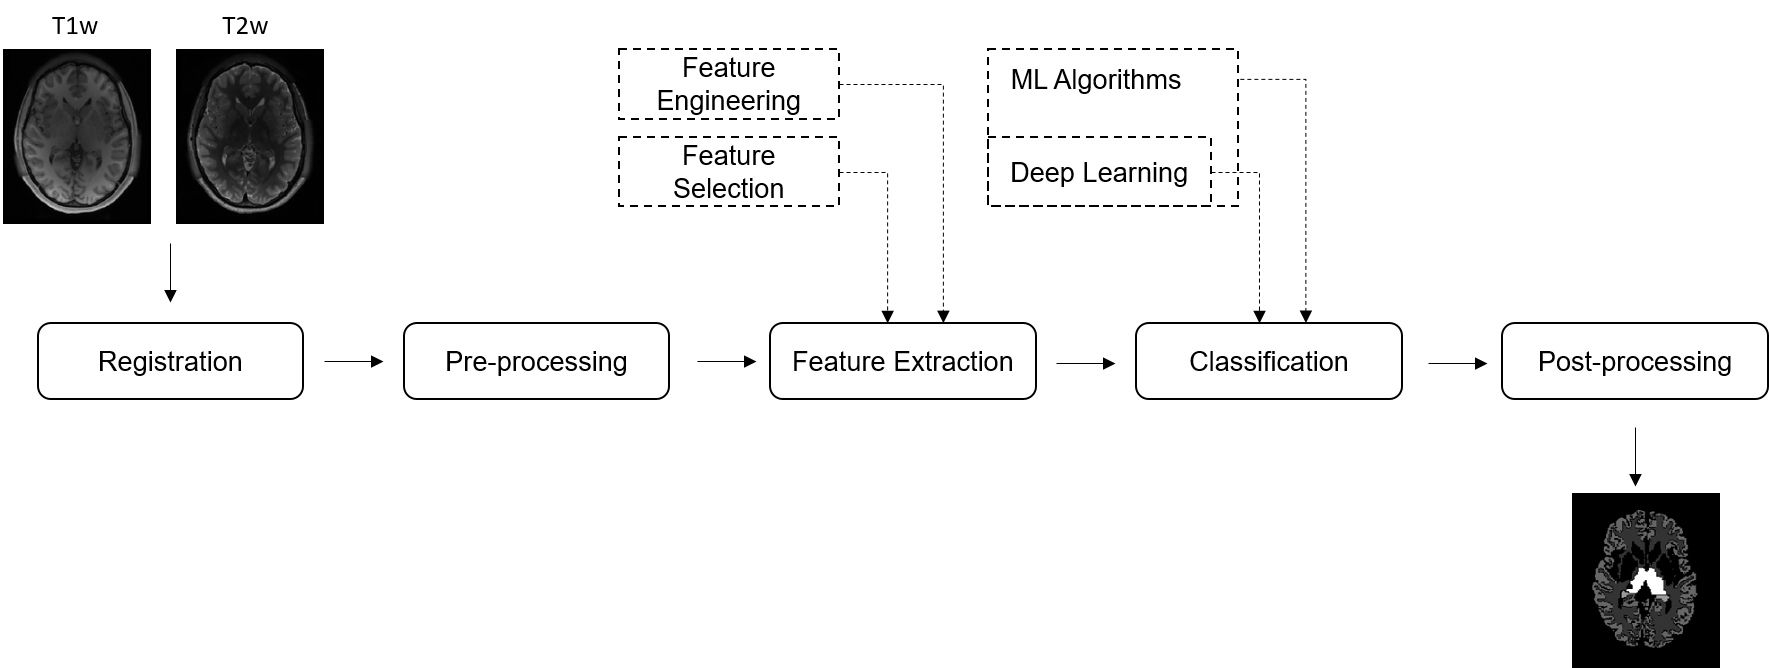
\includegraphics[width = .45 \textwidth]{img/pipeline}
	\caption{MIA pipeline}
	\label{fig:pipeline}
\end{figure}

Registration matches an acquired image to a reference one, usually provided from an atlas. This image transformation can be affine as well as non-rigid, which allows local deformations. The pre-processing is used to improve the quality of an image. It uses different kind of filters and masks to get a higher quality image or remove unnecessary data. Intensity normalization is also used, especially if machine learning is involved. Feature extraction tries to find position of anatomical landmarks. Contours and corners can be found with rather simple algorithms. Classification means to decide of the anatomical type for each voxel. This can be done in various ways, decisions trees (also called forests) in machine learning or by growing regions algorithms. Finally, post-processing gives a cleaner final segmentation. It will remove small groups of voxels that should not correspond to any real anatomical part. As an example, a human body can only have one liver or two kidneys of similar size.

To measure the overall performance, several evaluation metrics can be used. The Dice coefficient tells how good the computed result and the ground truth do overlap. It goes from 0 if there is no overlap at all to 1 being exactly same segmentation. The Hausdorff distance is another metric. It measures the maximum distance from the computed segmentation contour to the ground truth one. There are many more metrics that can be used to test specific parts of the computed segmentation.

\subsection*{Registration}
For the registration step, two different solutions have been compared. The first is affine transformation, which which allows translation, rotation and scaling. The second one is non-rigid, which transforms the volumes locally. This can lead to a better matching between the input image and the atlas. For the affine registration of two volumes, the volume to be registered is moved relative to the fixed volume by rotation, translation or scaling. After each displacement a similarity of the volumes is measured. This parameter is minimized by moving the volume further until a minimum is reached. The same is true for a non rigid registration, but there is an additional tuning factor which allows local displacements, rotations and scaling. We used the \textit{Simple Elastix}\footnote{\url{https://github.com/SuperElastix/SimpleElastix}} library to compute the non-rigid transformation. This library uses a B-spline registration to register the two volumes non rigidly.

\subsection*{Segmentation}
For the segmentation step, several types have been compared. The first one is machine learning based, essentially a random forest with 10 estimators of maximum depth of 40. The other methods were all atlas-based, where the weight function has been modified. The simplest one is when all images have the same weight. To reduce potentially worse ground truth inputs, we used global and local weights. In order to make the segmentation smoother, an additional method called Shape based averaging was implemented.

\subsubsection*{Machine Learning}
\subsubsection*{Majority Voting}
\subsubsection*{Global Weighted Voting}

\subsubsection*{Local Weighted Voting}
\subsubsection*{Shape Based Averaging}